\chapter{Конструкторский раздел}

В данном разделе будут приведены требования к входным, выходным параметрам и представлены схемы для алгоритмов линейного и бинарного поиска.

\section{Требования к входным и выходным параметрам}

Требования к входным и выходным параметрам:
\begin{itemize}[label=--]
    \item в качестве входных параметров алгоритм принимает массив и искомое значение;
    \item пустой массив является корректным входным значением;
    \item для бинарного поиска массив должен быть отсортирован;
    \item выходными параметрами являются два числа --- индекс искомого значения и количество сравнений, потребовавшихся для нахождения данного значения;
    \item если искомое значение не найдено, в качестве индекса возвращается $-1$.
\end{itemize}

\section{Линейный поиск}

На рисунке~\ref{fig:linear_search} представлена схема алгоритма линейного поиска.


\begin{figure}[!htb]
\centering
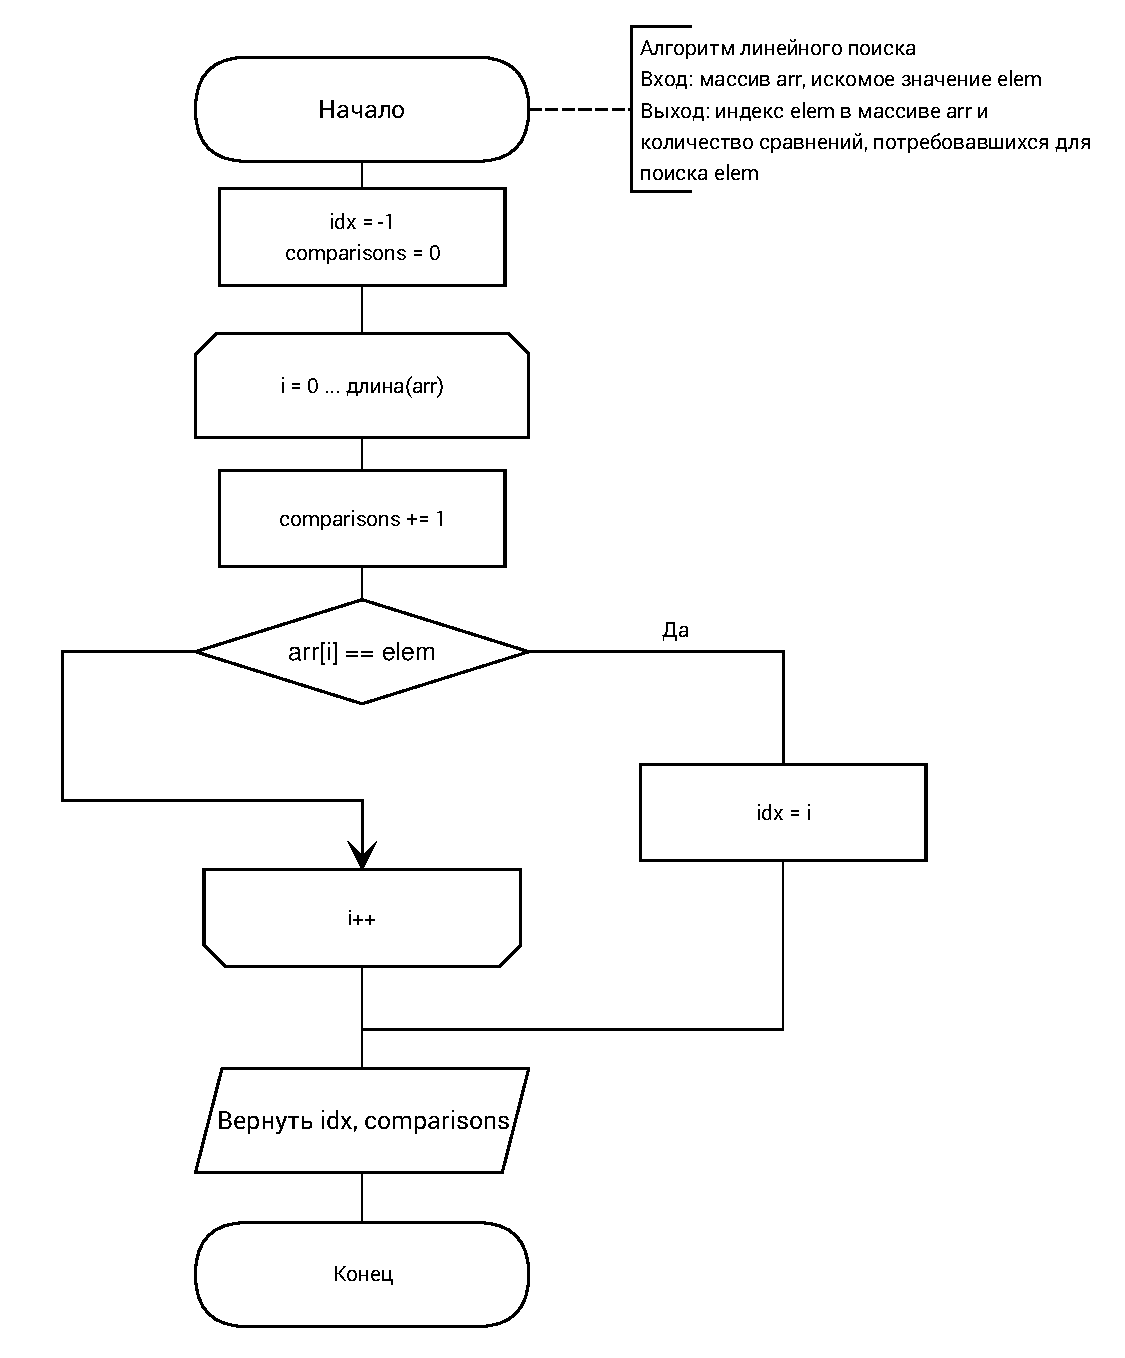
\includegraphics[width=\textwidth]{inc/img/linear_search.pdf}
\caption{Схема алгоритма линейного поиска}
\label{fig:linear_search}
\end{figure}

\section{Бинарный поиск}

На рисунке~\ref{fig:binary_search} представлена схема алгоритма бинарного поиска.

\begin{figure}[!htb]
\centering
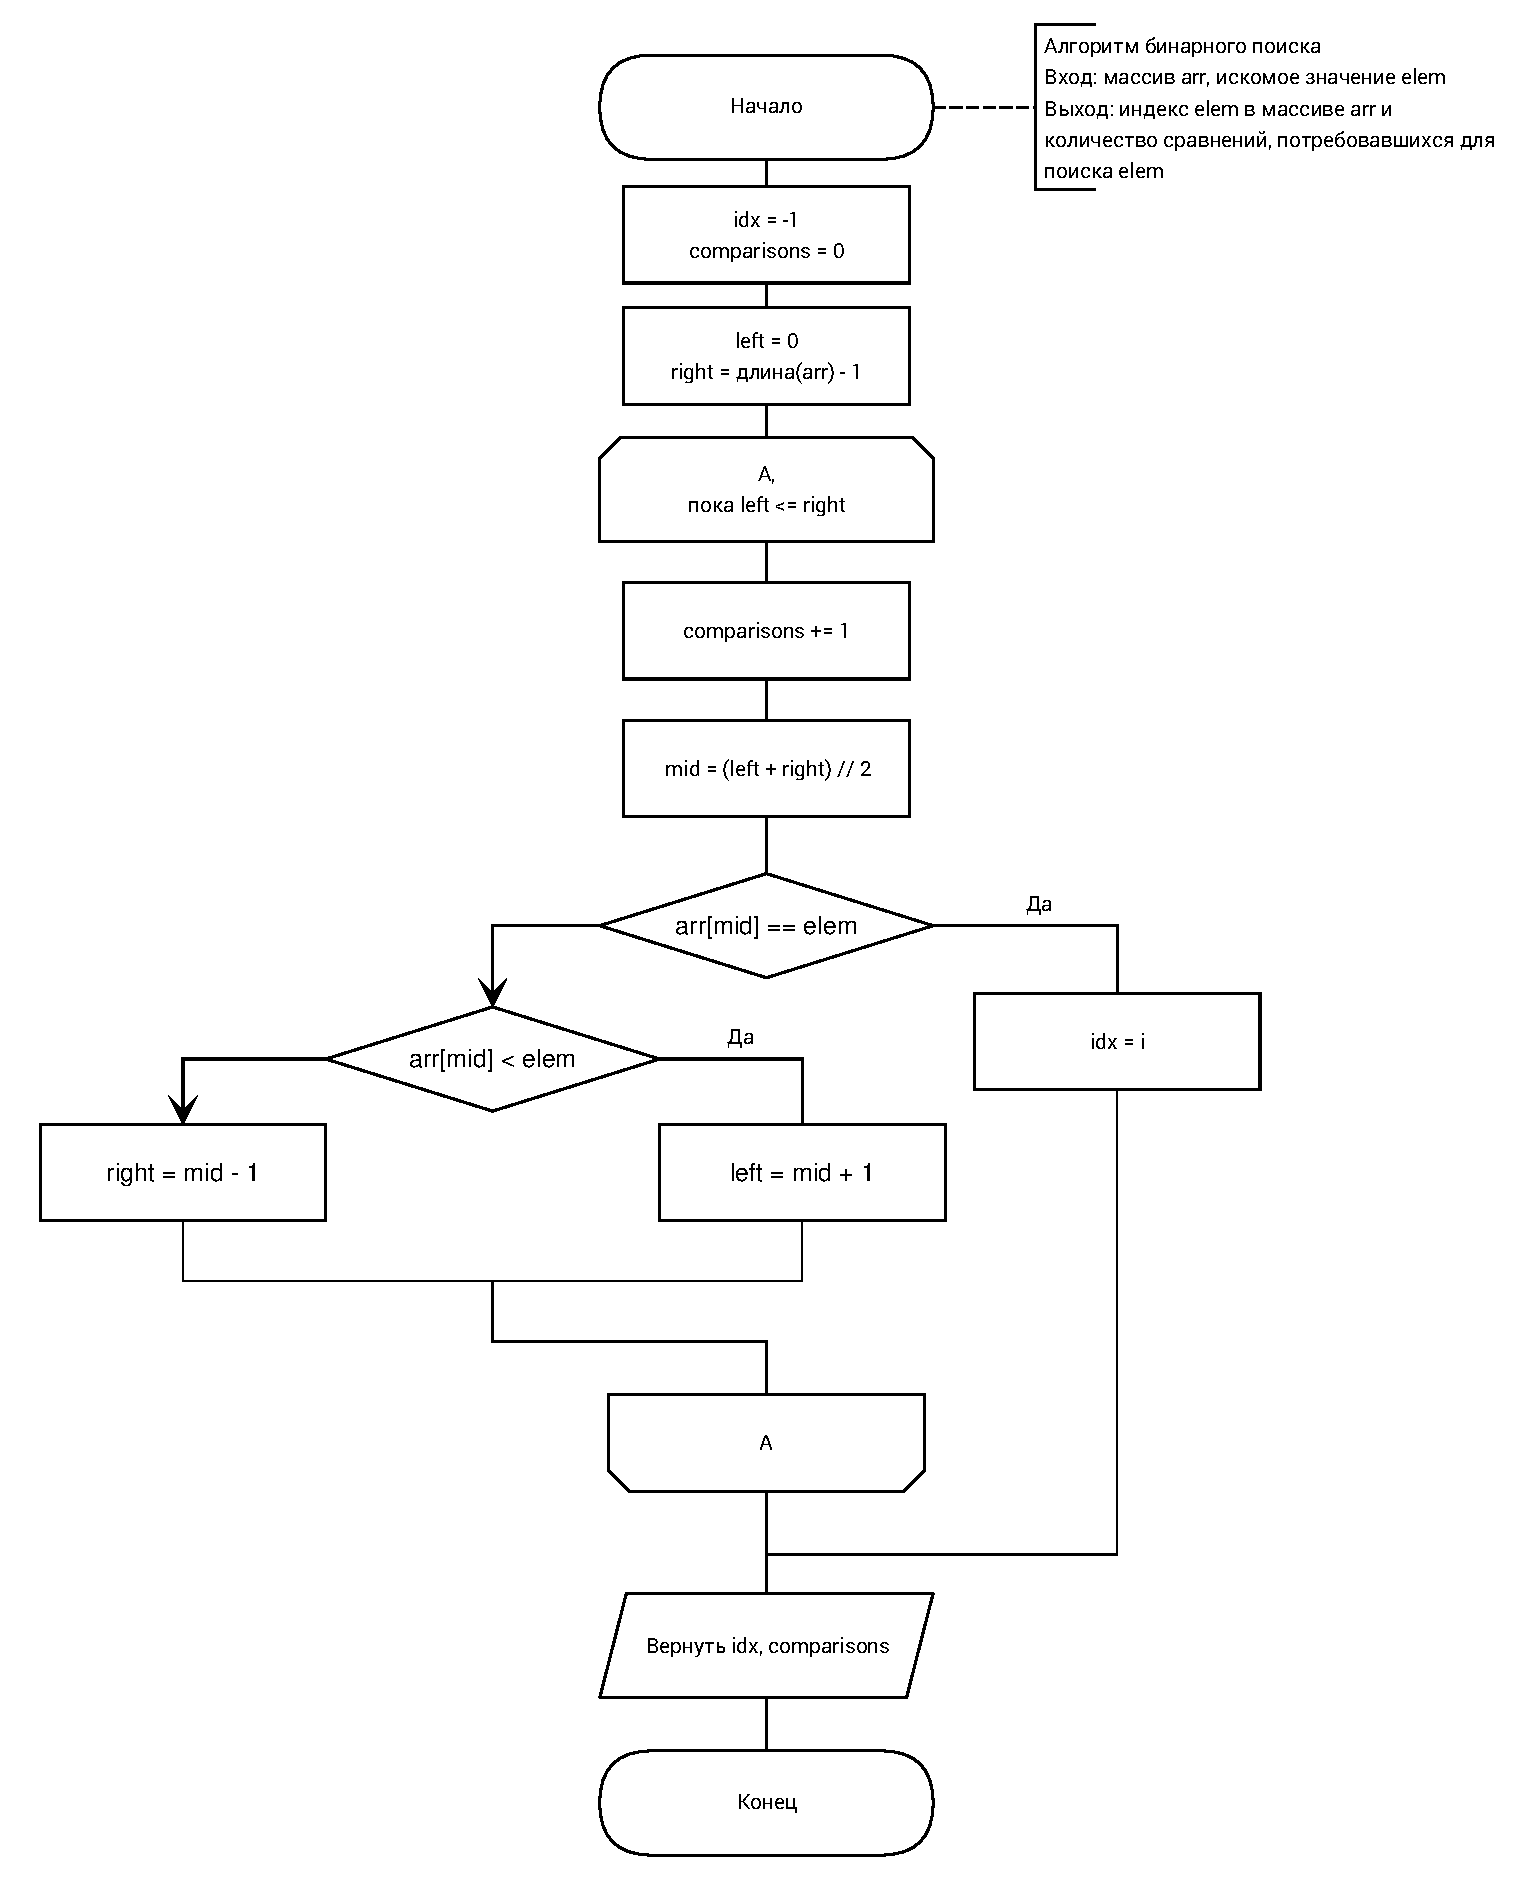
\includegraphics[width=\textwidth]{inc/img/binary_search.pdf}
\caption{Схема алгоритма бинарного поиска}
\label{fig:binary_search}
\end{figure}
